\documentclass[xcolor=svgnames]{beamer}

\usepackage{bera}
\usepackage[utf8]    {inputenc}
\usepackage[T1]      {fontenc}
\usepackage[english] {babel}

\usepackage{amsmath,amsfonts,graphicx}
\usepackage{beamerleanprogress}

\title
	[Escalabilidad de SDN en la RAU]
  {Proyecto de grado \\
  	Escalabilidad de Redes Definidas por Software en la Red Académica}

\author
	[Santiago Vidal]
  {Santiago Vidal \\
  	\vspace{4mm}
  	{\normalfont\small Tutores: \\
  	Dr. Eduardo Grampín \\
  	MSc. Martín Giachino}}

\date
  {5 de octubre de 2016}

\institute
  [UdelaR]
  {Instituto de Computación \\
  	Facultad de Ingeniería \\
  	Universidad de la República}


\begin{document}

% Directorio con las imagenes
\graphicspath{{Figs/}}

\maketitle

\begin{frame}{}
	\tableofcontents
\end{frame}

\section{Introducción}

\begin{frame}
	\tableofcontents[currentsection]
\end{frame}

\begin{frame}{Introducción}
	\begin{block}{Red Académica Uruguaya (RAU)}
		\begin{itemize}
			\item Emprendimiento de la Universidad de la República, administrado por el Servicio Central de Informática Universitario
			(SeCIU).
			\item Red que conecta instituciones académicas, centros de investigación e instituciones gubernamentales.
			\item Parte de la RedClara.
		\end{itemize}
	\end{block}
	\begin{block}{RAU2}
		RAU2 es un proyecto para reemplazar la infraestructura actual, con el objetivo de brindar más y mejores servicios a las instituciones.
	\end{block}
\end{frame}
%La idea de esta red es proveer servicios especializados para las insituciones, mayor calidad de servicio, mas velocidad, etc.
%Proveedores sobrevenden ancho de banda
%Actividades comerciales y particulares tienen misma prioridad.

\begin{frame}{Proyecto RRAP}
	\textbf{Routers Reconfigurables de Altas Prestaciones} (Emiliano Viotti, Rodrigo Amaro):
	\begin{itemize}
		\item Proyecto de grado que terminó en agosto de 2015.
		\item Construyó un prototipo para la RAU2, basado en SDN.
		\item Desarrolló una aplicación para gestión de redes llamada \textbf{RAUFlow}, que implementa clasificación y separación de tráfico.
	\end{itemize}
\end{frame}

\begin{frame}{Proyecto RRAP}
	\begin{center}
		Prototipo físico para pruebas funcionales:
		\begin{figure}[t]
			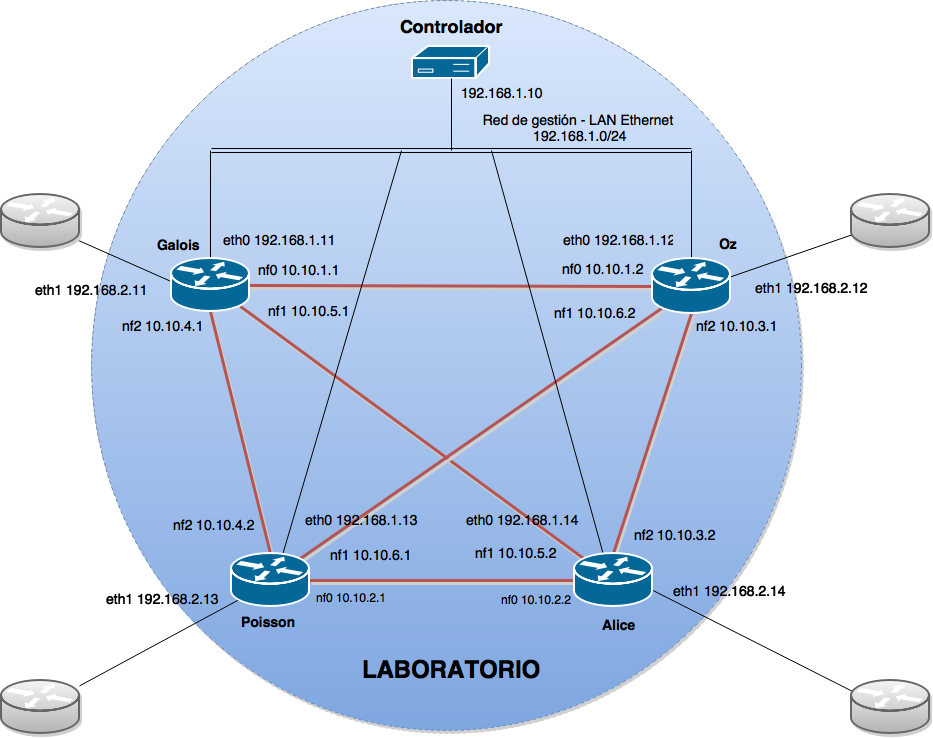
\includegraphics[scale=0.25]{topologia_rrap}
		\end{figure}
	\end{center}
\end{frame}

\begin{frame}{Motivación}
	Contestar las siguientes preguntas:
	\pause
	\begin{enumerate}
		\item ¿Cómo podemos seguir trabajando sobre la arquitectura RAUflow sin ser limitados por el prototipo físico?
		\pause
		\item ¿RAUFlow funciona con topologias más grandes?
		\pause
		\item ¿Tiene buena escalabilidad?
		%en el contexto de la RAU, es vital estudiar la escalabilidad de cualquier enfoque porque va a afectar a muchas instituciones, usuarios y tráfico.
	\end{enumerate}
\end{frame}

\begin{frame}{Resultados esperados}
	\pause
	\begin{enumerate}
		\item Estado del arte en las aplicaciones de SDN (con foco en VPNs), y las herramientas de virtualización disponibles.
		\pause
		\item Una herramienta que permita virtualizar la arquitectura RAUFlow para pruebas y desarrollo.
		\pause
		\item Diseño e implementación de pruebas para estudiar la escalabilidad de RAUFlow.
	\end{enumerate}
\end{frame}

\section{Conceptos previos \& RAUFlow}

\begin{frame}{}
	\tableofcontents[currentsection]
\end{frame}

\begin{frame}{Diapo1}
	
\end{frame}

\section{Entorno virtual}

\begin{frame}{}
	\tableofcontents[currentsection]
\end{frame}

\begin{frame}{Objetivo}
	Poder utilizar la arquitectura RAUFlow y RAUSwitch en un entorno virtual para:
	\begin{itemize}
		\item Experimentos y pruebas.
		\item Desarrollo de nuevas funcionalidades sobre RAUFlow.
		\item Investigación sobre esquemas híbridos en general.
	\end{itemize}
\end{frame}
%Pruebas y experimentos que no son posibles con prototipos físicos. Incluso si se contara con todo el equipamiento, la configuración es muy compleja.

\begin{frame}{Requerimientos}
	Requerimientos funcionales:
	\begin{enumerate}
		\item RAUSwitch virtuales:
		\begin{enumerate}
			\item OpenFlow 1.3
			\item OSPF
			\item SNMP (no esencial)
		\end{enumerate}
		\item Hosts virtuales
		\item Controlador RAUFlow
	\end{enumerate}
	\pause
	Requerimientos no funcionales:
	\begin{enumerate}
		\item Configurabilidad / Usabilidad
		\item Escalabilidad
	\end{enumerate}
\end{frame}

\begin{frame}{Siguiente paso}
	\begin{center}
		Se descarta una construcción desde cero
	\begin{figure}[t]
		
\includegraphics[scale=0.1]{arrow_down}
	\end{figure}
	Hay que encontrar una herramienta que cumpla los requerimientos
	\end{center}
\end{frame}

\begin{frame}{Elección de una herramienta}
	\begin{alertblock}{Herramientas orientadas a SDN}
		\begin{itemize}
			\item Algunas no soportan OpenFlow 1.3
			\item Algunas no permiten un controlador externo.
			\item \textbf{Ninguna contempla switches híbridos!}
		\end{itemize}
	\end{alertblock}
	\pause
	\begin{block}{Herramientas de propósito general}
		\begin{itemize}
			\item Algunas no tienen buena configurabilidad.
			\item La \textbf{escalabilidad} es un gran problema.
		\end{itemize}
	\end{block}
\end{frame}

\begin{frame}{Mininet}
	\begin{itemize}
		\item Emulador de redes.
		\item Comúnmente utilizado para experimentar con SDN y OpenFlow.
		\item Ofrece Hosts y Switches.
		\item Virtualización ligera (containers).
		\item Cumple todos los requerimientos \textbf{excepto} el soporte para switches híbridos.
		\item Pero permite al usuario definir sus propias clases de nodos para extender las funcionalidades de las clases que vienen por defecto.
	\end{itemize}
\end{frame}

\begin{frame}{Arquitectura de Mininet}
	\begin{figure}[t]
		\centering
		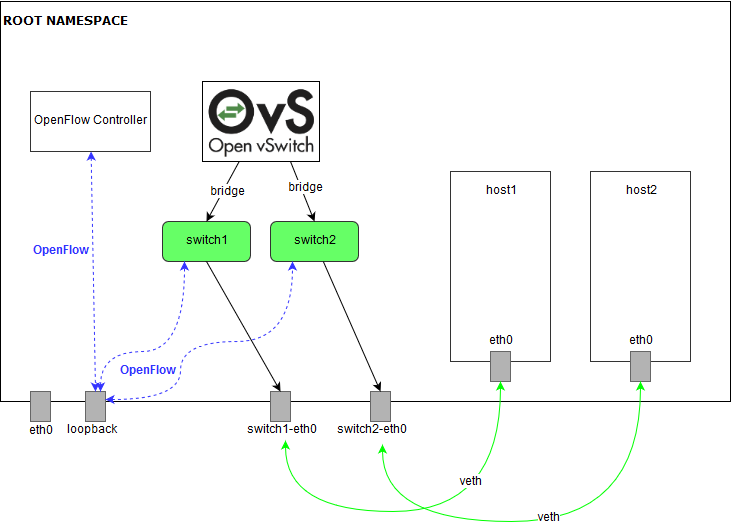
\includegraphics[scale=0.5]{mininet_architecture}
	\end{figure}
\end{frame}
% Los recursos de red de cada switch no están aislados entre sí.

\begin{frame}{Problema con Mininet tradicional}
	\begin{itemize}
		\item Los switches están en el root namespace, así que no es posible que cada uno ejecute su instancia de Quagga.
		\item No es posible poner a cada Switch en su propio namespace ya que Open vSwitch no tendría acceso a ellos.
		\item Si los switches están en su propio namespace, el controlador OpenFlow (RAUFlow) no puede comunicarse con ellos a través de la interfaz de loopback.
	\end{itemize}
	\pause
	{\color{green}Solución: utilizar Mininet pero como emulador de propósito general.}
\end{frame}

\begin{frame}{Diseño de la solución}
	\begin{figure}[t]
		\centering
		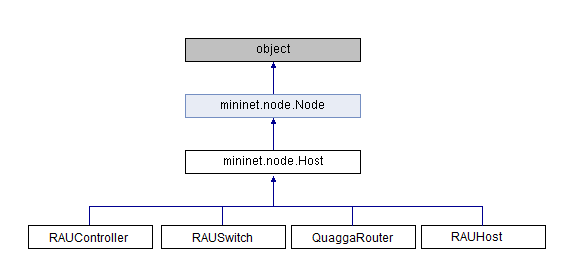
\includegraphics[scale=0.7]{clases_entorno}
	\end{figure}
\end{frame}

\begin{frame}{Arquitectura del entorno construido}
	\begin{figure}[t]
		\centering
		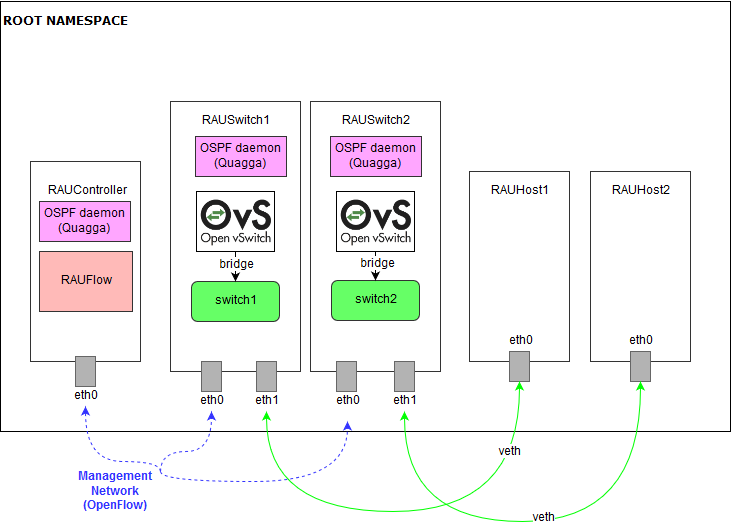
\includegraphics[scale=0.5]{emulator_architecture}
	\end{figure}
\end{frame}
%Aca mencionar que OVS es el aspecto mas radical, y que resulta complejo ejecutar multiples instancias correctamente (capaz mencionar que es gracias a privateDirs, capaz).

\begin{frame}{Eliminación de SNMP}
	\begin{figure}[t]
		\centering
		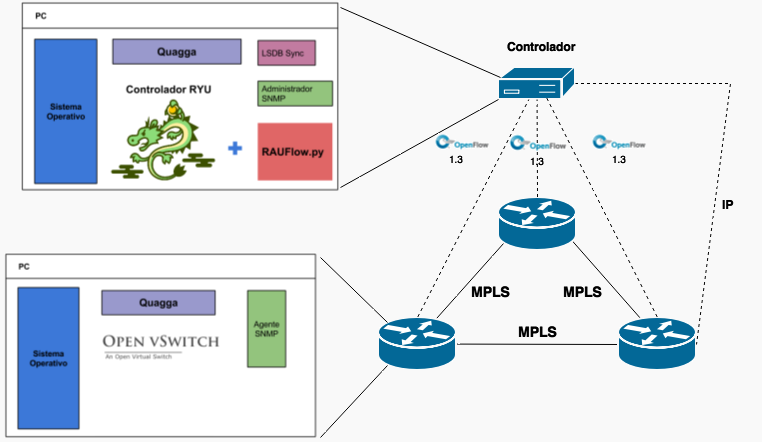
\includegraphics[scale=0.5]{componentes_rauflow}
	\end{figure}
\end{frame}

\begin{frame}{Eliminación de SNMP}
	\begin{figure}[t]
		\centering
		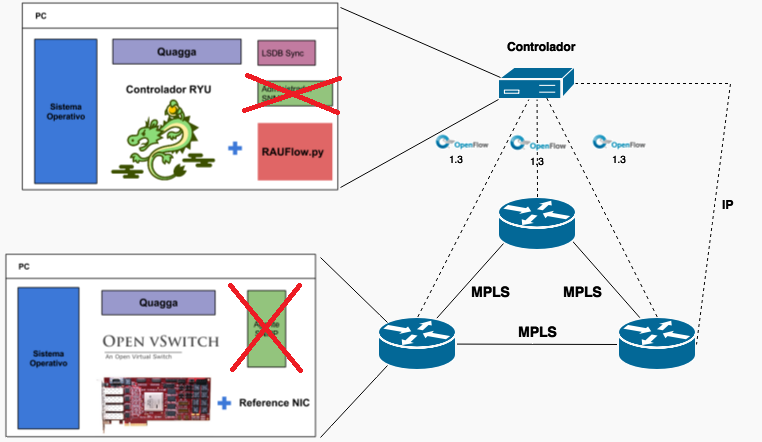
\includegraphics[scale=0.5]{componentes_rauflow_2}
	\end{figure}
\end{frame}

\begin{frame}{Eliminación de SNMP}
	El envío de datos de las interfaces pasa a implementarse con Open vSwitch (por fuera de OpenFlow).
	\begin{exampleblock}{Ventajas}
		\begin{itemize}
			\item Reduce complejidad de la arquitectura.
			\item Reduce carga de cómputo en los switches.
		\end{itemize}
	\end{exampleblock}
\end{frame}

\begin{frame}{Verificación funcional}
	Con el entorno construido, el siguiente paso es probar distintos escenarios y topologias para detectar:
	\begin{itemize}
		\item Problemas con el entorno virtual.
		\item Problemas con la arquitectura/código de RAUFlow.
	\end{itemize}
\end{frame}

\begin{frame}{Problemas encontrados}
	\begin{enumerate}
		\item \textbf{Error en el código de RAUFlow}: error en el algoritmo del camino óptimo. Provocaba una excepción de Python.
		\item \textbf{Error en el código de RAUFlow}: error en el código que instala los flujos OpenFlow en los nodos. Provocaba que los flujos en cada nodo de un camino tuvieran incorrecto puerto de entrada.
	\end{enumerate}
\end{frame}

\begin{frame}{Problemas encontrados}
	\begin{enumerate}
		\setcounter{enumi}{2}
		\item \textbf{Posible problema} en el módulo LSDB Sync para leer base de datos topológica de OSPF cuando la topología es muy grande (librería Telnetlib de Python).
		\item \textbf{Posible problema} de comunicación en la red de gestión cuando hay muchos switches.
	\end{enumerate}
\end{frame}

\begin{frame}{Problemas encontrados}
	\begin{figure}[t]
		\centering
		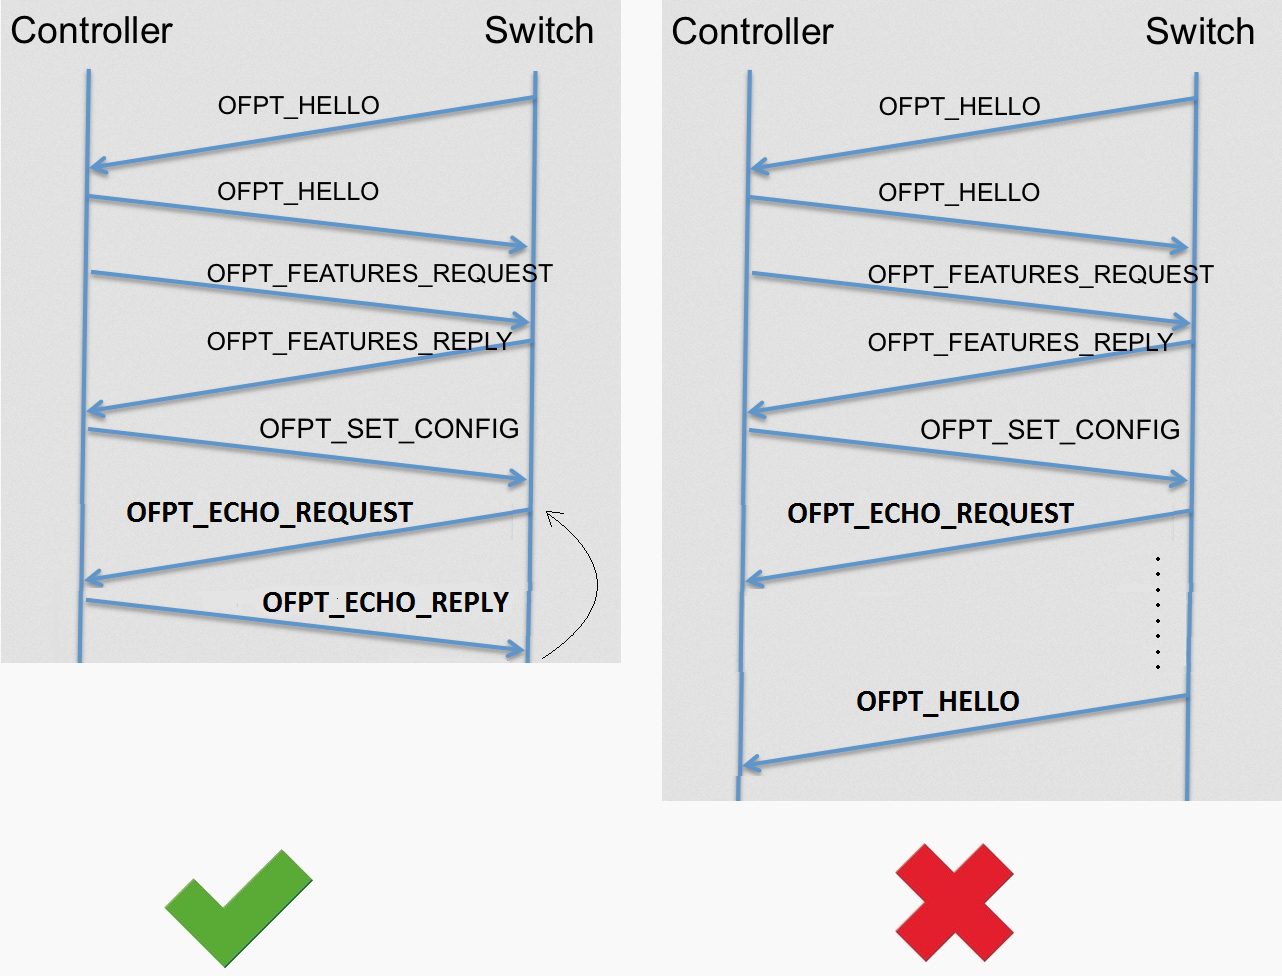
\includegraphics[scale=0.3]{openflow_protocol_error}
	\end{figure}
\end{frame}

\section{Pruebas de escala}

\begin{frame}{}
	\tableofcontents[currentsection]
\end{frame}

\begin{frame}{Diapo1}
	
\end{frame}

%Utiliza las mismas herramientas que el prototipo físico, lo cual mejora la calidad de los experimentos. También implica que podría utilizarse en conjunto con dispositivos físicos.




\section{Conclusiones}

\begin{frame}{}
	\tableofcontents[currentsection]
\end{frame}

\begin{frame}{Diapo1}
	
\end{frame}

\end{document}

